
The chosen setup consists of a VM spun up with a vulnerable image from Pentesterlab\cite{pentesterlab}. The VM has an apache server hosting a web application that uses a bash-based CGI script. The topology can be seen on figure \ref{fig:network-topology}. 
\begin{figure} [ht]
    \centering
    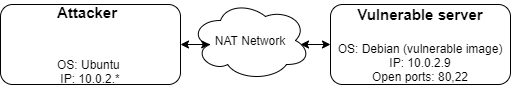
\includegraphics[width=\columnwidth]{drawio/topology.png}
    \caption{Environment topology}
    \label{fig:network-topology}
\end{figure} 

The server has bash version 4.2.45(1)-release installed, which is a version vulnerable to shellshock. Furthermore the web application is hosted on port 80. 




 